\par This section describes the variables used in the $\nu_e$ selections to isolate features that are specific to events with final-state electrons. We split these variables in several categories according to the pertinence of the calorimetric or topological information used: Slice Variables, Shower, Track, Shower and Track, and Shower/Track-like  Classification Variables,  2nd Shower-Based $\pi^0$ Rejection Variables.  While Table~\ref{tab:variableSummary} summarizes all variables used with a brief description, variables that warrant a longer introduction are described below. In the following, we define the leading track (shower) as the track (shower) with the most hits.

\par \noindent  \textbf{Slice Variables}: these variables describe general features of the reconstructed neutrino interaction or event.
\par \noindent  \textbf{Track Variables}: these variables describe the features of track objects.
\begin{itemize}
 \item[] \textbf{Track PID} (variable: \texttt{trkpid}).  This variable is the LLR-PID (sec.~\ref{subsec:loglikelihoodpid}) score for the longest track in the slice. -1 is proton-like, 1 is muon-like. 
 \end{itemize}
%\par \noindent \textbf{Shower Variables}:  these variables describe the features of shower objects.
\par \noindent \textbf{Track-Shower Distance Variables}: these variables are used to measure the separation in space between the leading shower and the leading track, for events where at least one track and one shower are present in the slice. 
\begin{itemize}
 \item[] \textbf{3D track-shower distance} (variable: \texttt{tksh\_distance}).  This variable is the 3D distance between the shower start point and the reconstructed start point of the longest track in the slice. 
 \item[] \textbf{2D track-shower distance} (variable: \texttt{trkshrhitdist2}) Due to mis-reconstruction in the 3D shower and track reconstruction, sometimes the 3D distance is significantly smeared (up to several centimeters) even if the individual track and shower are correctly clustered. These factors decrease the track-shower separation of $\nu_e$ interactions therefore reducing the $e-\gamma$ separation power achievable. To overcome this failure a new quantity is calculated with 2D information from the collection plane defined as the smallest 2D distance between any hits associated with the shower candidate and any hits associated with the proton candidate. This variable is therefore complementary to the quantity \texttt{tksh\_distance}.
\end{itemize}



\par \noindent \textbf{Shower/Track-like  Classification Variables}: The first step in track-shower classification relies on the topological score reconstructed by Pandora (variable: \texttt{shr\_score}), which utilizes inputs such as the PCA component of 3D space-points to classify PFParticles. Nonetheless, this classification is not sufficient to obtain the track-shower separation needed. To improve on this, additional variables which leverage different aspects of shower topologies are devised:

\begin{itemize}

    \item[] \textbf{Shower Track-Fitted Fraction} (variable: \texttt{trkfit}, figure~\ref{fig:nue:variables:trkfit}) This quantity is the fraction of the 3D spacepoints in a shower object that are successfully fit with the shower track-fitter algorithm. Tracks, comprised of a single contiguous segment, will be entirely fit, leading to a fraction of 1. Showers, with several branches and split charge deposition segments, will have a fraction that is less then one.
    \item[] \textbf{Shower Sub-Clusters} (variable: \texttt{subcluster}, figure~\ref{fig:nue:variables:subcluster}) This quantity leverages the fact that EM showers are often comprised of several branches isolated by gaps caused by photons propagating through the detector medium. The variable is calculated by counting the number of isolated 2D segments of charge associated with reconstructed showers. This quantity is a sum of such clusters from all three planes.
    \item[] \textbf{Moliere ``Angle''} (variable: \texttt{shrmoliereavg}) This quantity aims to characterize the profile of reconstructed EM showers. It is computed using 3D spacepoints. For each 3D spacepoint, the angle between the shower's direction and the spacepoint is calculated. The average of all such angles is used as the variable.
    \item[] \textbf{shower track-fitted length} (variable: \texttt{shr\_trk\_len}, discussed in sec.~\ref{sec:sideband:newcuts:shrtrklen}) the length of the shower using the start- and end-points obtained by fitting the PFParitcle under the track hypothesis.
    \item[] \textbf{Cylindrical Fraction} (variable: \texttt{CylFrac2h\_1cm}) This variable measures the fraction of spacepoints of the leading shower that are within 1 cm of the shower central axis. Only the second half of the PFParticle is considered for this calculation, where showers are expected to lead to a low fraction of well-aligned spacepoints, and tracks to a high fraction.
    \item[] \textbf{Shower Principal Component Median} (variable: \texttt{shrPCA1CMed\_5cm}) The aim of this variable is to assess the linearity of a shower. It is calculated by breaking up the leading shower into segments of 5 cm and performing a principle component analysis (PCA) on each segment. Then, for each segment, the ratio of the first component eigenvalue and the sum of the eigenvalues is calculated. The median of the ratios is taken.
    \item[] \textbf{Shower Delta RMS} (variable: \texttt{DeltaRMS2h}) The aim of this quantity is to measure the spread of the shower along the axis orthogonal to shower direction. This is determined by performing a PCA on the shower spacepoints and calculating the RMS for the second component.
    Only the second half of the shower is considered.
    \item[] \textbf{Shower Multiple Coulomb Scatering (MCS) Momentum} (variable: \texttt{shrMCSMom}) This quantity characterizes the spread of the leading shower taking into account the separation of each 3D spacepoint to the center of the shower as well as the length of the shower and doing a MCS momentum calculation on the shower. For details see reference~\cite{bib:baller}.
    \item[] \textbf{dE/dx Variables} (fig.~\ref{fig:nue:variables:dedx}) These variables are computed using calorimetric information as described in sec.~\ref{subsec:egammaspearation}. Three sets of variables are calculated as the median d$E$/d$x$ computed over different segment of a shower's trunk: $[0,2]$, $[1,5]$, and $[0,4]$ cm. The variable \texttt{shr\_tkfit\_gap10\_dedx\_\{U,V,Y\}} which skips the first cm of shower trunk from the d$E$/d$x$ calculation is motivated by cases where the first few hits of a shower merge activity from short protons, causing a large d$E$/d$x$ which hampers the ability to identify the shower as an electron. These cases are particularly relevant as backgrounds for the \zpsel channel. The variable \texttt{shr\_tkfit\_2cm\_dedx\_\{U,V,Y\}} which focuses on the very first segment of ionization tries to leverage the fact that for photon showers the d$E$/d$x$ becomes more and more MIP-like as one moves further along the shower, especially at low energy (see figure~\ref{fig:dedxgammas:dist}). Information from the different planes is further condensed into a single variable, \texttt{shr\_tkfit\_dedx\_max}, which is computed to be the d$E$/d$x$ value on the plane with the largest number of hits in the $[0,4]$ cm range of the shower trunk.
\end{itemize}{}

\begin{figure}[H] 
\begin{center}
    \begin{subfigure}[b]{0.27\textwidth}
    \centering
    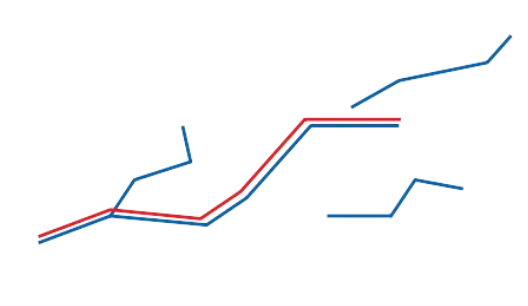
\includegraphics[width=1.00\textwidth]{nueselection/variables/trkfit.png}
    \caption{\label{fig:nue:variables:trkfit} ``trkfit'' variable }
    \end{subfigure}
    \begin{subfigure}[b]{0.27\textwidth}
    \centering
    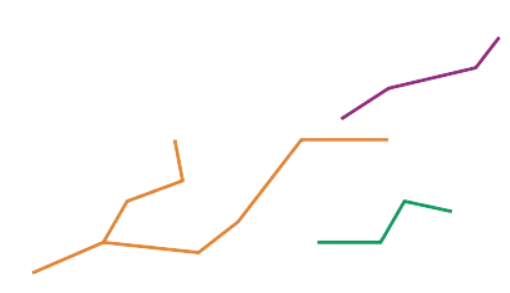
\includegraphics[width=1.00\textwidth]{nueselection/variables/nbranch.png}
    \caption{\label{fig:nue:variables:subcluster} ``subcluster'' variable }
    \end{subfigure}
    \begin{subfigure}[b]{0.27\textwidth}
    \centering
    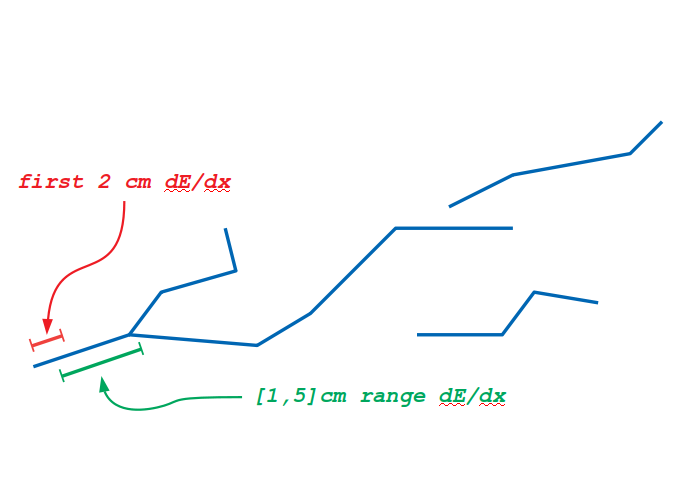
\includegraphics[width=1.00\textwidth]{nueselection/variables/dedx.png}
    \caption{\label{fig:nue:variables:dedx} d$E$/d$x$ variables }
    \end{subfigure}
\caption{\label{fig:nue:presel:eff} Additional shower variables defined by the analysis to improve track-shower separation.}
\end{center}
\end{figure}

\par \noindent  \textbf{Second Shower Based $\pi^0$ Rejection Variables}: %Often, one of the two EM $\gamma$ showers in $\pi^0$ events is not fully reconstructed by Pandora. In many cases, these second $\gamma$ showers are correctly identified by Pandora as belonging to the neutrino slice (reconstructed in 2D), but never fully reconstructed in 3D (see fig.~\ref{fig:nue:variables:secondshowerevd}).
Pandora's reconstruction of events containing $\pi^0$s is often imperfect. In many cases, both EM $\gamma$ showers are correctly identified as belonging to the same neutrino slice (reconstructed in 2D), but one of the showers is not fully reconstructed in 3D (see fig.~\ref{fig:nue:variables:secondshowerevd}).

To improve on our $\pi^0$ rejection, we build several variables storing information associated to the largest 2D cluster on each plane included in the neutrino-slice, but not reconstructed as a full 3D particle. The variables, shown graphically in figure~\ref{fig:nue:variables:secondshower}, are described in Table ~\ref{tab:variableSummary}. In the example event of Figure~\ref{fig:nue:variables:secondshowerevd}, these quantities are computed for the circled black cluster of charge which represents a missed photon in the $\pi^0$ reconstruction.

\begin{figure}[H] 
\begin{center}
    \begin{subfigure}[b]{0.27\textwidth}
    \centering
    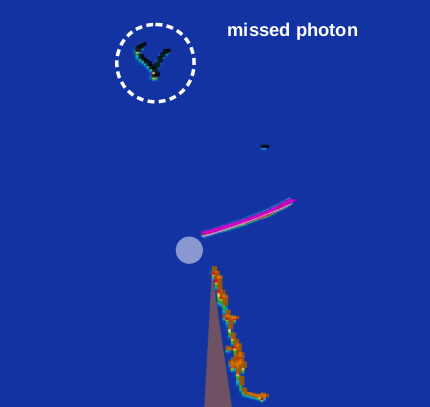
\includegraphics[width=1.00\textwidth]{nueselection/variables/secondshowerevd.png}
    \caption{\label{fig:nue:variables:secondshowerevd} unclustered shower }
    \end{subfigure}
    \begin{subfigure}[b]{0.27\textwidth}
    \centering
    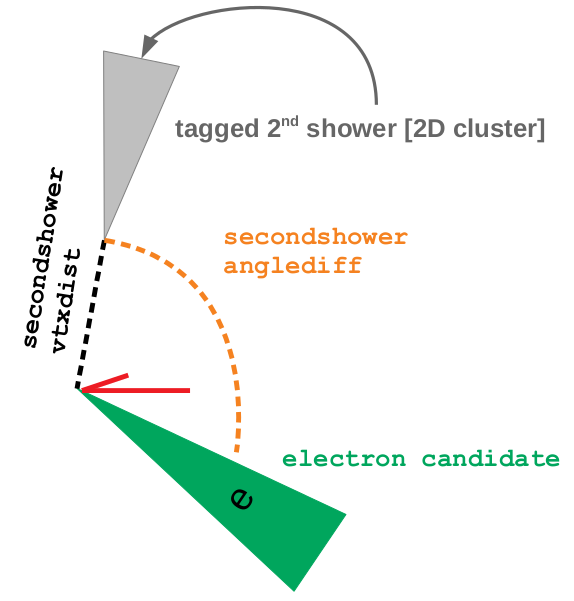
\includegraphics[width=1.00\textwidth]{nueselection/variables/secondshower.png}
    \caption{\label{fig:nue:variables:secondshower}second-shower variables }
    \end{subfigure}
\caption{\label{fig:nue:variables:secondshower} Visual representation of the second shower based $\pi^0$ rejection variables. Left: example event where the second shower in a $\pi^0$ event is clustered in 2D (black hits) but not fully reconstructed in 3D. Right: reconstructed variables associated with the second-shower search. The gray cone in the image represents the black cluster on the left image, for which only 2D information is accessible.}
\end{center}
\end{figure}

%\par \noindent  \textbf{Shower Dispersion Variables}: These variables are used to characterize the geometry of the leading shower, using as inputs the 3D space-points. 


\begin{table}[ht]
\caption{\label{tab:variableSummary} Summary of the definitions for the variables used in the analysis.}
\centering
\begin{tabular}{ m{0.07\textwidth} | m{0.28\textwidth} | m{0.6\textwidth}  }
Category & Variable Name & Description  \\
\hline

\multicolumn{1}{l|}{} & \texttt{nslice} &  Number of neutrino slices identified by the \texttt{SliceID}. Values are  0 or 1.\\  \cline{2-3}
\multicolumn{1}{l|}{} & \texttt{reco\_nu\_vtx\_sce\_\{x,y,z\}} & Reconstructed neutrino interaction vertex in (x,y,z) coordinates. The space charged correction is applied.  \\  \cline{2-3}
\multicolumn{1}{l|}{} & \texttt{n\_showers\_contained} & Number of showers with a starting point within the fiducial volume. \\  \cline{2-3}
\multicolumn{1}{l|}{} & \texttt{n\_tracks\_contained} & Number of tracks fully contained in the fiducial volume.  \\  \cline{2-3}
\multicolumn{1}{l|}{} & \texttt{n\_tracks\_tot} & Total number of tracks in the event; contained or exiting.  \\  \cline{2-3}
\multicolumn{1}{l|}{} & \texttt{contained\_fraction} & Hits in PFParticles contained in the fiducial volume over the total number of clustered hits in the slice.  \\  \cline{2-3}
\parbox[t]{2mm}{\multirow{4}{*}{\rotatebox[origin=c]{90}{Slice}}} & \texttt{hits\_ratio} & Ratio between hits from showers and total number of hits in the slice. \\  \cline{2-3}
\multicolumn{1}{l|}{} & \texttt{CosmicIP} & Closest distance between shower start and space points associated to tracks flagged as cosmics. \\  \cline{2-3}
\multicolumn{1}{l|}{} & \texttt{crtveto} & Boolean variable checking if the event passes the CRT veto. \\  \cline{2-3}
\multicolumn{1}{l|}{} & \texttt{\_closestNuCosmicDist} &  3D distance between the reconstructed neutrino vertex and the closest CRT-tagged cosmic track. \\  \cline{2-3}
\multicolumn{1}{l|}{} & \texttt{slclustfrac} & Fraction of hits in the slice that are fully reconstructed to 3D particles. \\  \cline{2-3}
\multicolumn{1}{l|}{} & \texttt{shr\_trk\_sce\_\{start,end\}\_y} &  Start and end point in y of shower when fit as a track.    \\ \cline{2-3}
\multicolumn{1}{l|}{} & \texttt{nObjHits\_\{U,V,Y\}} & Number of hits associated with the object on each plane.\\  
\hline
\parbox[t]{2mm}{\multirow{8}{*}{\rotatebox[origin=c]{90}{Track, Shower Separation}}}  &
 \texttt{pfp\_generation} & The generation of the PFParticle according to Pandora: the neutrino has generation 1, it's direct daughters 2, and further decay products 3 or higher.\\  \cline{2-3}
\multicolumn{1}{l|}{} & \texttt{trkpid}  &  Proton-muon LLR particle identification. \\  \cline{2-3}
%\multicolumn{1}{l|}{} & \texttt{ismerged} & Check if a proton is merged at the beginning of a shower.\\ \cline{2-3}
\multicolumn{1}{l|}{} & \texttt{shr\_energy\_tot\_cali}  & Sum  of  the  energy  of  the  calibrated  showers  (in  GeV). Used  only  at pre-selection as a ``Michel veto”.\\  \cline{2-3}
\multicolumn{1}{l|}{} & \texttt{shr\_score} & Pandora  SVM track/shower score for the leading shower.\\  \cline{2-3}
\multicolumn{1}{l|}{} & \texttt{tksh\_angle}  & Angle  between  leading  shower   and  longest  track directions.\\  \cline{2-3}
%\multicolumn{1}{l|}{} & \texttt{merge\_bestdist}  & Distance between shower start point and track start (or end) point for the track in the slice that best matches the direction of the shower.\\  \cline{2-3}
\multicolumn{1}{l|}{} & \texttt{trfit} & Fraction of the 3D spacepoints successfully fitted with the shower track-fitter algorithm. \\  \cline{2-3}
\multicolumn{1}{l|}{} & \texttt{subcluster} & Number of isolated 2D segments of charge associated to a reconstructed shower on all three planes.  \\  \cline{2-3}
\multicolumn{1}{l|}{} & \texttt{shrmoliereavg} &  Average angle between the shower’s direction and its 3D spacepoints.    \\ \cline{2-3}
\multicolumn{1}{l|}{} & \texttt{shr\_trk\_len} &  Length of shower when fit as a track.    \\ \cline{2-3}
\multicolumn{1}{l|}{} & \texttt{tk1sh1\_angle\_alltk} &  Angle between shower and exiting track.    \\ \cline{2-3}
\multicolumn{1}{l|}{} & \texttt{CylFrac2h\_1cm} & Fraction of spacepoints in a 1 cm cylinder around the second half of the shower.   \\ \cline{2-3}
\multicolumn{1}{l|}{} & \texttt{shrPCA1CMed\_5cm} & Median PCA component calculated in 5 cm blocks.  \\ \cline{2-3}
\multicolumn{1}{l|}{} & \texttt{DeltaRMS2h} & RMS of spacepoint distance from shower center in the second half of the shower.  \\ \cline{2-3}
\multicolumn{1}{l|}{} & \texttt{shrMCSMom} & Multiple Coulomb scattering shower momentum.  \\ 
\hline
\multicolumn{1}{l|}{} & \texttt{shr\_tkfit\_gap10\_dedx\_\{U,V,Y\}}  & Median dE/dx computed over [1,5] cm of the shower’s  trunk. \\ \cline{2-3}
\multicolumn{1}{l|}{} & \texttt{shr\_tkfit\_2cm\_dedx\_\{U,V,Y\}}  & Median dE/dx computed  over  the first 2 cm of the shower’s  trunk. \\ \cline{2-3}
\parbox[t]{2mm}{\multirow{4}{*}{\rotatebox[origin=c]{90}{$e$/$\gamma$ Separation}}}  & \texttt{shr\_tkfit\_dedx\_\{U,V,Y\}}  & Median dE/dx computed  over  the first 4 cm of the shower’s  trunk. \\ \cline{2-3}
\multicolumn{1}{l|}{} & \texttt{shr\_tkfit\_dedx\_max, shr\_tkfit\_2cm\_dedx\_max}  & Median dE/dx on plane with most number of hits in $[0,4], [0,2]$ cm trunk segment. \\ \cline{2-3}
\multicolumn{1}{l|}{} & \texttt{shower\_vtx\_dist} & Distance between the shower start and the neutrino vertex.\\ \cline{2-3}
\multicolumn{1}{l|}{}  & \texttt{tksh\_distance}  & Distance between leading shower and longest track start points in 3D.\\  \cline{2-3}
\multicolumn{1}{l|}{}  & \texttt{trkshrhitdist2}  & Minimum distance between leading shower and longest track clusters in 2D.\\  
\hline
\multicolumn{1}{l|}{} & \texttt{secondshower\_\{U,V,Y\}\_nhit} & Number of hits on each plane of the largest cluster associated with the  recovered 2nd shower  \\  \cline{2-3}
\parbox[t]{2mm}{\multirow{4}{*}{\rotatebox[origin=c]{90}{Second Shower}}}  & \texttt{secondshower\_\{U,V,Y\}\_dot} &  Dot product between the vector connecting the vertex to the closest hit in cluster and the charge-weighted cluster direction w.r.t. closest hit in cluster \\  \cline{2-3}
\multicolumn{1}{l|}{} & \texttt{anglediff\_\{U,V,Y\}} & 2D angle difference in each plane between the 2nd shower and the 1st shower cluster  (cluster direction defined as charge-weighted direction of cluster w.r.t. vertex) \\ \cline{2-3}
\multicolumn{1}{l|}{} & \texttt{secondshower\_\{U,V,Y\}\_vtxdist} & 2D distance from vertex for the largest 2D cluster associated with the recovered 2nd shower in each plane \\ 
\hline
\end{tabular}
\label{tab:variableSummary}
\end{table}
